\subsection{满射性判别法}

命题 4. --- 设 E、F 是两个 Fréchet 空间，u 是 E 到 F 中的一个连续线性映射。下列条件等价：

\begin{enumerate}
\def\labelenumi{(\roman{enumi})}
\item
  u 是满射。
\item
  对每个半范数 \(p \in \mathbf{S}(\mathbf{E})\)，存在 \(q \in \mathbf{S}(\mathbf{F})\)，使得不等式 \(|f| \leqslant q\) 对每个线性型 \(f \in \mathbf{F}'\)（满足 \(|f \circ u| \leqslant p\) 者）都成立。
\item
  对每个半范数 \(p \in \mathrm{S}(\mathrm{E})\)，存在 \(q \in \mathrm{S}(\mathrm{F})\) 满足下列性质：若线性型 \(f \in F'\) 满足 \(|f \circ u| \leqslant p\)，则 f 在 q 为零的点上为零，并且对所有 \(y \in F\)、\(r \in \mathrm{S}(\mathrm{F})\)，存在 \(x \in E\) 使得 \(r(u(x) - y) = 0\)。
\item
  对每个半范数 \(p \in \mathrm{S}(\mathrm{E})\)，我们有
\end{enumerate}

\[
\sup_{\substack{f\in \mathbf{F}^{\prime}\\ |f\circ u|\leqslant p}}\big|f(y)\big| <   + \infty \quad \text{对所有} \quad y\in \mathbf{F}  .\tag{1}
\]

我们将按照下面的逻辑图式来证明该命题

\pandocbounded{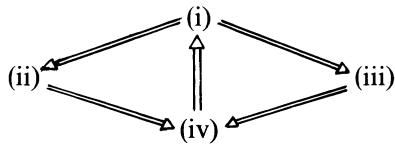
\includegraphics[keepaspectratio]{images/part002_fd83f186.jpg}}

若 \(u\) 是满射，则它是一个严格态射 (IV, 第 28 页, 定理 1)，于是对每个半范数 \(p \in \mathrm{S}(\mathrm{E})\)，存在半范数 \(q \in \mathrm{S}(\mathrm{F})\)，使得对所有 \(y \in \mathrm{F}\)（满足 \(q(y) \leqslant 1\) 者），存在 \(x \in \mathrm{E}\) 满足 \(p(x) \leqslant 1\) 且 \(u(x) = y\)。我们立即推出 (i) 蕴含 (ii) 与 (iii)。显然 (ii) 蕴含 (iv)。

为证 (iii) 蕴含 (iv)，设 \(p\) 与 \(q\) 如 (iii) 所述。设 \(y \in \mathbf{F}\)，由 (iii)，存在 \(x\)（属于 \(\mathbf{E}\)）使得 \(q(u(x) - y) = 0\)。若 \(f \in \mathbf{F}'\) 满足 \(|f \circ u| \leqslant p\)，则有 \(f(u(x) - y) = 0\)，于是

\[
\left| f (y) \right| = \left| f (u (x)) \right| \leqslant p (x)
\]

从而关系式 (1) 成立。

最后证明 (iv) 蕴含 (i)。设 \(p \in \mathrm{S}(\mathrm{E})\)，设 \(q\) 是诸函数 \(|f|\)（\(f \in \mathrm{F}'\) 取遍满足 \(|f \circ u| \leqslant p\) 者）的上包络。由 (iv)，\(q\) 在 \(\mathrm{F}\) 上有限，且显然是 \(\mathrm{F}\) 上的一个下半连续半范数；由于 \(\mathrm{F}\) 是桶型空间 (III, 第 25 页, 推论)，我们有 \(q \in \mathrm{S}(\mathrm{F})\)。设 \(\mathbf{B}_p\)（相应地，\(\mathbf{B}_q\)）表示所有 \(x \in \mathrm{E}\)（相应地，\(y \in \mathrm{F}\)）中满足 \(p(x) \leqslant 1\)（相应地，\(q(y) \leqslant 1\)）者所成的集。我们有 \(q \circ u \leqslant p\)，于是 \(u(\mathbf{B}_p) \subset \mathbf{B}_q\)。\(u(\mathbf{B}_p)\) 在 \(\mathrm{F}'\) 中的极集由这样的线性型 \(f \in \mathrm{F}'\) 组成：它们满足 \(|f \circ u| \leqslant p\)，从而 \(|f| \leqslant q\)；换句话说，我们得到 \(u(\mathbf{B}_p)^{\circ} \subset \mathbf{B}_q^{\circ}\)，最后，\(\overline{u(\mathbf{B}_p)} = \mathbf{B}_q\) 由双极定理 (II, 第 45 页, 推论 3) 得出。若 \(\mathrm{U}\) 是 \(\mathrm{E}\) 中 0 的一个邻域，则存在 \(p \in \mathrm{S}(\mathrm{E})\) 使得 \(\mathbf{B}_p \subset \mathbf{U}\)，于是 \(\overline{u(\mathbf{U})}\) 包含邻域 \(\mathbf{B}_q\)（即 \(\mathrm{F}\) 中 0 的邻域）。这就蕴含 \(u\) 是满射 (I, 第 17 页, 定理 1)。

推论. --- 设 E 与 F 是 Banach 空间。下列条件等价：

\begin{enumerate}
\def\labelenumi{(\roman{enumi})}
\item
  \(u\) 是满射。
\item
  存在实数 \(r > 0\)，使得 \(\| f \| \leqslant r\) . \(\| {}^t u(f) \|\) 对所有 \(f \in \mathbf{F}'\) 成立。
\item
  对所有 \(y \in F\)，我们有 \(\sup_{\substack{f\in \mathbf{F}^{\prime}\\ |f\circ u|\leqslant 1}} |f(y)| < +\infty\)。
\end{enumerate}

条件 (ii) 与 (iii) 实际上就是命题 4 的条件 (ii) 与 (iv) 在 Banach 空间情形下的重新表述。

